\section{Objective}
\begin{itemize}
	\item To understand the core principles of network reduction using Thevenin's theorem in linear, bilateral DC circuits.
	\item To construct a multi-resistor DC network and measure its open-circuit voltage ($V_{th}$) and equivalent resistance ($R_{th}$).
	\item To verify experimentally that the original network and its single-source Thevenin equivalent deliver identical current and voltage to a load.
	\item To evaluate agreement between empirical laboratory data and theoretical network calculations.
\end{itemize}

\section{Introduction}
Analyzing load response variations in complex networks becomes computationally repetitive if the complete circuit must be re-solved for every load modification. Thevenin's Theorem addresses this by modeling any two-terminal linear network—regardless of internal complexity—as a single equivalent voltage source connected in series with an equivalent resistance. This experiment demonstrates Thevenin's theorem by assembling a DC network, determining its equivalent parameters, and demonstrating terminal equivalence across a load resistor.

\section{Theory}

\subsection{Thevenin's Theorem}
Thevenin's Theorem states that any two-terminal, linear, bilateral DC network containing voltage sources and resistors can be represented by an equivalent circuit comprising an independent voltage source ($V_{th}$) in series with an equivalent resistor ($R_{th}$).
\begin{itemize}
	\item \textbf{Thevenin Voltage ($V_{th}$):} The open-circuit voltage measured across terminal pair A--B when load $R_L$ is removed.
	\item \textbf{Thevenin Resistance ($R_{th}$):} The equivalent resistance measured looking back into terminals A--B with all independent voltage sources replaced by short circuits (\qty{0}{\volt}).
\end{itemize}
Connected to load $R_L$, the load current $I_L$ and terminal voltage $V_L$ follow:
\[
I_L = \frac{V_{th}}{R_{th}+R_L}, \qquad V_L = I_L R_L.
\]

\subsection{Relation to Norton's Theorem}
Norton's Theorem offers a dual representation: replacing the network with an equivalent current source $I_N$ in parallel with $R_N$, where $R_N = R_{th}$ and $V_{th} = I_N R_N$.

\section{Apparatus and Components}
\begin{table}[h!]
	\centering
	\caption{List of Equipment and Components Used}
	\vspace{2mm}
	\begin{tabular}{llc}
		\toprule
		\rowcolor{blue!10}
		\textbf{Item Description} & \textbf{Specification / Rating} & \textbf{Quantity} \\
		\midrule
		DC Power Supply & \qty{15}{\volt} regulated & 1 \\
		Resistor $R_1$ & \qty{670}{\ohm} & 1 \\
		Resistor $R_2$ & \qty{670}{\ohm} & 1 \\
		Resistor $R_3$ & \qty{670}{\ohm} & 1 \\
		Load Resistor $R_L$ & \qty{970}{\ohm} & 1 \\
		Digital Multimeter (DMM) & DC Voltage / Current / Ohms & 1 \\
		Solderless Breadboard & Standard Tie-Point & 1 \\
		Connecting Wires & Jumper Wires & As required \\
		\bottomrule
	\end{tabular}
	\label{tab:apparatus4}
\end{table}

\section{Circuit Diagram}

\subsection{Original Circuit}
\begin{figure}[h!]
	\centering
	\begin{circuitikz}[american, scale=1.0]
		\draw (0,0) to[battery1, l={$V=\qty{15}{\volt}$}, invert] (0,3)
		(0,3) to[R, l=$R_1$] (4,3)
		to[R, l=$R_2$] (8,3)
		to[ammeter, l=$A$] (8,1.5)
		to[R, l=$R_L$] (8,0) -- (0,0);
		\draw (4,3) to[R, l=$R_3$] (4,0);
		\draw (4,0) node[ground]{};
		\draw (8,0) node[ground]{};
		\node at (6,3.3) [above] {A};
		\node at (8,-0.4) [below] {B};
	\end{circuitikz}
	\caption{Original DC network featuring $R_1=R_2=R_3=\qty{670}{\ohm}$ and load $R_L=\qty{970}{\ohm}$ driven by $V=\qty{15}{\volt}$.}
	\label{fig:theveninoriginal}
\end{figure}

\subsection{Thevenin Equivalent Circuit}
\begin{figure}[h!]
	\centering
	\begin{circuitikz}[american, scale=1.0]
		\draw (0,0) to[battery1, l=$V_{th}$, invert] (0,3)
		(0,3) to[R, l=$R_{th}$] (4,3)
		to[R, l=$R_L$] (4,0) -- (0,0);
		\draw (4,0) node[ground]{};
	\end{circuitikz}
	\caption{Thevenin equivalent circuit driving load $R_L$ via series parameters $V_{th}$ and $R_{th}$.}
	\label{fig:theveninequiv}
\end{figure}

\section{Experimental Procedure}

\subsection*{Part A: Original Circuit Measurement}
\begin{enumerate}
	\item Assemble the primary circuit on the breadboard (Figure~\ref{fig:theveninoriginal}) with load $R_L$ across terminals A--B.
	\item Record load voltage ($V_L$) and current ($I_L$) using the digital multimeter.
\end{enumerate}

\subsection*{Part B: Verification of Thevenin's Theorem}
\begin{enumerate}
	\item Disconnect load resistor $R_L$ from terminals A--B.
	\item Measure open-circuit voltage across terminals A--B to determine $V_{th}$.
	\item Deactivate the DC source (short-circuiting supply terminals) and measure terminal resistance across A--B using an ohmmeter to determine $R_{th}$.
	\item Build the equivalent model (Figure~\ref{fig:theveninequiv}) on a separate breadboard section using $V_{th}$ and $R_{th}$.
	\item Connect load $R_L$ across the equivalent circuit and record resulting load parameters.
\end{enumerate}

\section{Theoretical Calculation}
With load $R_L$ removed, open-circuit output matches the voltage division across $R_3$:
\[
V_{th} = V\left(\frac{R_3}{R_1+R_3}\right).
\]
With source $V$ short-circuited, equivalent input resistance equals $R_1 \parallel R_3$ in series with $R_2$:
\[
R_{th} = R_2 + \left(\frac{R_1 R_3}{R_1+R_3}\right).
\]
Theoretical load parameters are computed as:
\[
I_L = \frac{V_{th}}{R_{th}+R_L}, \qquad V_L = I_L R_L.
\]

\section{Data Collection}
\begin{table}[h!]
	\centering
	\caption{Experimental Data for the Verification of Thevenin's Theorem}
	\vspace{2mm}
	\begin{tabular}{lcccc}
		\toprule
		\rowcolor{blue!10}
		\textbf{Parameter} & \textbf{Original Circuit} & \textbf{Thevenin Equiv.} & \textbf{Theoretical} & \textbf{\% Error} \\
		& \textbf{(measured)} & \textbf{(measured)} & \textbf{Value} & \\
		\midrule
		Open-Circuit Voltage, $V_{th}$ & N/A & \qty{8.23}{\volt} & \qty{8.105}{\volt} & 1.54\% \\
		Equivalent Resistance, $R_{th}$ & N/A & \qty{1.03}{\kilo\ohm} & \qty{978}{\ohm} & 5.3\% \\
		Load Current, $I_L$ & \qty{4}{\milli\ampere} & \qty{4.02}{\milli\ampere} & \qty{4.16}{\milli\ampere} & 3.37\% \\
		Load Voltage, $V_L$ & \qty{4}{\volt} & \qty{4.07}{\volt} & \qty{4.0352}{\volt} & 0.86\% \\
		\bottomrule
	\end{tabular}
	\label{tab:thevdata}
\end{table}

\section{Result Analysis}
Measured parameters ($V_{th}=\qty{8.23}{\volt}$, $R_{th}=\qty{1.03}{\kilo\ohm}$) showed close agreement with theoretical values (\qty{8.105}{\volt}, \qty{978}{\ohm}), yielding minor percentage errors of $1.54\%$ and $5.3\%$. Original load metrics ($I_L=\qty{4}{\milli\ampere}$, $V_L=\qty{4}{\volt}$) closely matched parameters recorded from the physical equivalent circuit ($I_L=\qty{4.02}{\milli\ampere}$, $V_L=\qty{4.07}{\volt}$), confirming electrical equivalence.

\section{Discussion and Sources of Error}
Experimental deviations are mainly attributed to:
\begin{enumerate}
	\item \textbf{Resistor Tolerances:} Variance between coded and real resistance values influences both $R_{th}$ measurements and theoretical outputs.
	\item \textbf{Contact Resistance:} Contact resistance within breadboard strips and shorting links slightly shifts ohmmeter resistance readings.
	\item \textbf{Multimeter Burden Voltage:} Ammeter internal resistance introduces minor loading effects during branch current readings.
	\item \textbf{Equivalent Parameter Substitution:} Practical component tolerances prevent exact matching of calculated $R_{th}$ on physical breadboards.
\end{enumerate}

\section{Conclusion}
The experimental results validate Thevenin's Theorem within small operational error limits. The physical equivalent network replicated terminal behavior effectively, proving that a complex linear network can be reduced to a single source with series resistance.

\section{References}
\begin{tcolorbox}[colback=gray!5, colframe=gray!40, arc=2mm]
	\begin{enumerate}
		\item Alexander, C. K., \& Sadiku, M. N. O. (2016). \textit{Fundamentals of Electric Circuits} (6th ed.). McGraw-Hill Education.
		\item Hayt, W. H., Kemmerly, J. E., \& Durbin, S. M. (2012). \textit{Engineering Circuit Analysis} (8th ed.). McGraw-Hill Education.
		\item Boylestad, R. L. (2015). \textit{Introductory Circuit Analysis} (13th ed.). Pearson.
	\end{enumerate}
\end{tcolorbox}

\section{Lab Data Sheet}
\begin{center}
	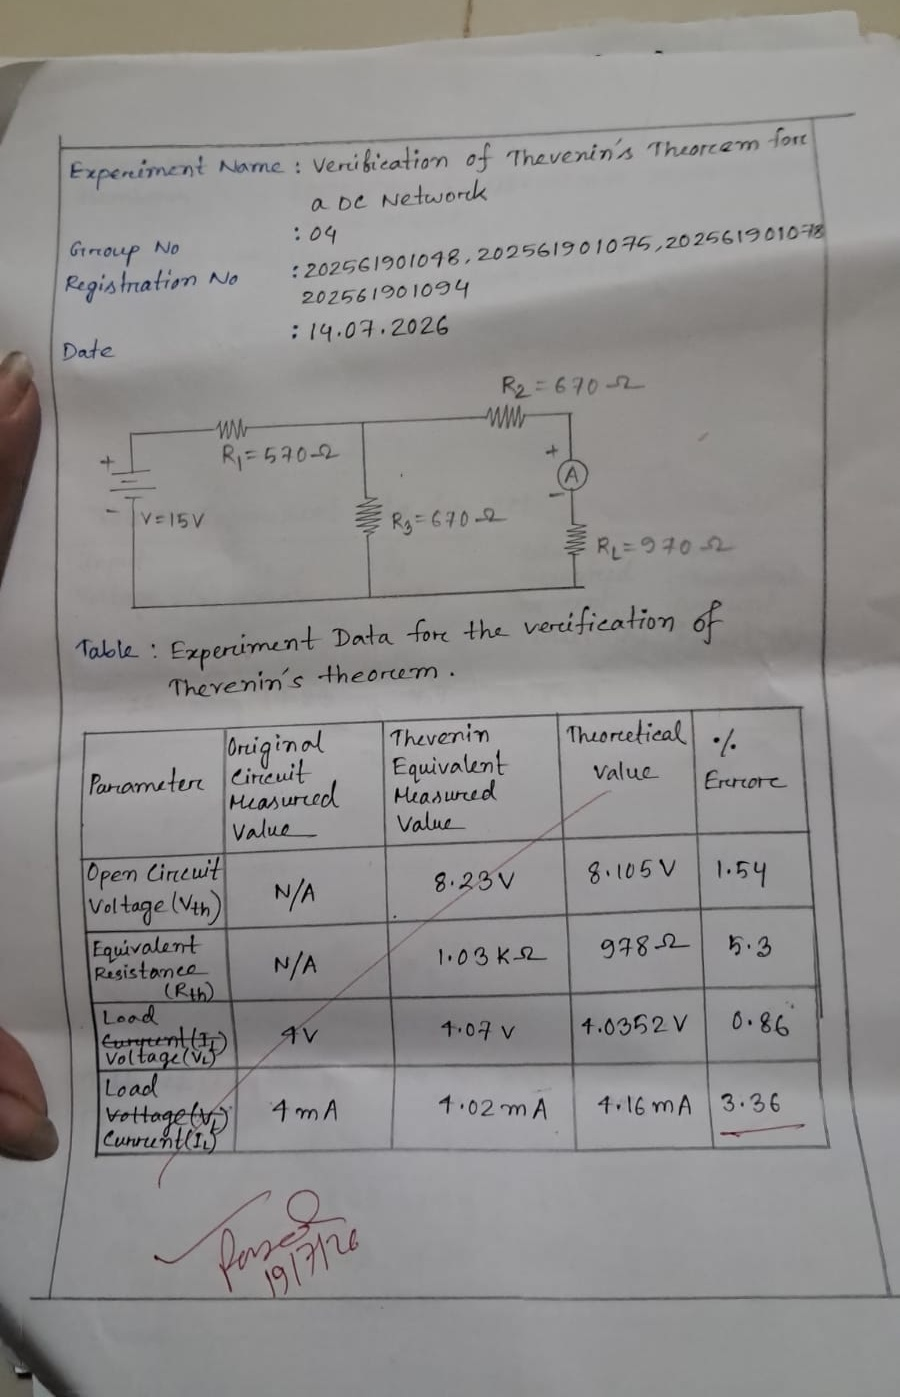
\includegraphics[width=0.95\textwidth, height=0.70\textheight, keepaspectratio]{datasheet2.png}
	
	\vspace{2mm}
	\small\textbf{Figure 3: Handwritten Lab Data Sheet for Experiment 04}
\end{center}